\begin{frame}{Active Learning}
    \begin{itemize}
        \item A system attempts to learn the label of an observation by enabling users catalog unlabeled observations \cite{report:active-learning}
        \item Aims to learn relationship among observations/labels using as few observations as possible
    \end{itemize}
\end{frame}


\begin{frame}{Active Learning}
    \begin{figure}[H]
      \centering
      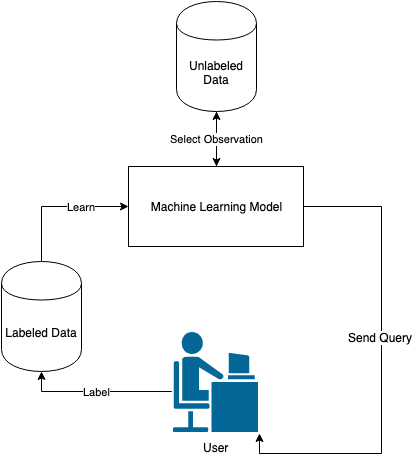
\includegraphics[
            height=0.6\textheight,
            keepaspectratio
      ]{report/images/active-learning.png}
      \caption{Diagram illustration of a possible active learning setup which relies in a user to label data.}
      \label{fig:active-learning}
    \end{figure}
\end{frame}